% \documentclass[a4paper]{article}
% \usepackage[ngerman]{babel}
% \usepackage[utf8]{inputenc}
% \usepackage[top=2.5cm,bottom=1.75cm,right=2cm,left=2.3cm]{geometry}
% \usepackage{wrapfig}
% \usepackage{floatflt}
% \usepackage{graphicx}
% \usepackage{subfigure}
% \usepackage[colorlinks=true,linkcolor=black,bookmarksnumbered=true,breaklinks=true,pdfstartview=FitH]{hyperref}
% 
% \title{\textbf{Praktikum 8} \\ ~ \\Schallgeschwindigkeit in Luft und Messing}
% 
% \author{Michael Kopp}
% 
% \date{17. Juli 2007}
% 
% \begin{document}
% 
% \maketitle


		\section{Versuch}



In ein Glasrohr werden feine Korkspäne gegeben und gleichmäßig verteilt. Dann sorgt man dafür, dass eine Schallwelle in das Rohr gelangt. Dort wird sie an den Rohrenden reflektiert. Um die Art der Reflexion zu beeinflussen, kann man eine der Öffnungen oder beide verschließen. Um die Länge des Rohres, in dem die Schallwellen schwingen können, zu beeinflussen, kann man einen der beiden Stopfen weiter nach innen oder außen bewegen.


\begin{figure}[h]
	\centering
	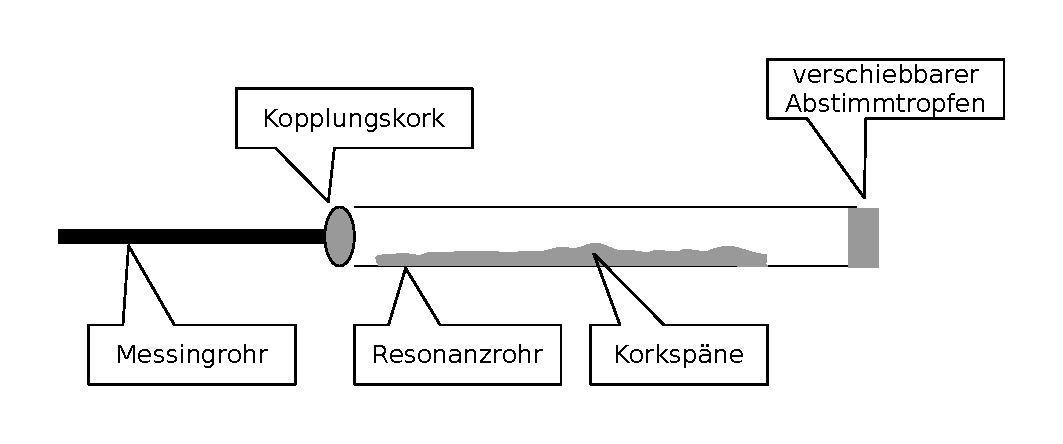
\includegraphics[width=0.8\textwidth]{praktika/mat_praktika/aufbau}
	\caption{Skizze des Versuchsaufbaus - sowohl das Messingrohr mit Kopplungskork als auch der Abstimmstopfen sind entfernbar.}
\end{figure}
Die Schallwellen werden dabei erzeugt durch 
\begin{enumerate}
	\item eine Stimmgabel 
	\item ein Messingrohr, an dem mit einem feuchten Lappen gerieben wird (dessen Schallwellen werden über ein \textit{Kopplungskork} an einem Ende der Röhre an die Luft im Rohr abgegeben)
	\item einen Lautsprecher, der mit einem Sinusgenerator betrieben wird
\end{enumerate}

Die Idee dahinter ist, dass sich in dem Rohr eine \textit{Stehende Welle} bildet. Diese hat dann \textit{Bewegungsbäuche}. Diese liegen immer an der selben Stelle und können hier die Korkspäne bewegen. An diesen Stellen werden die Korkspäne deshalb bald verschwunden sein, weil die Schallwellen sie immer in Längsrichtung zum Rohr bewegen. Sie sammeln sich dann an Stellen, an denen die Luft sich nicht (oder wenig) bewegt. Diese Stellen werden als \textit{Geschwindigkeitsknoten} bezeichnet.




		\section{Schallgeschwindigkeit in Luft}
		\label{kap:c_luft}



Das Resonanzrohr wird an einem Ende mit dem Abstimmstopfen verschlossen, dann wird eine Stimmgabel angeschlagen. Sei wird vor das offene Ende gehalten und der Abstimmstopfen wird so lange in das Resonanzrohr hineingeschoben bzw. herausgezogen, bis die Korkspäne sich zu kleinen Hügelchen anordnen - bis sich also eine \textit{stehende Welle} gebildet hat.

Bei dem Versuch wurde dabei eine Stimmgabel verwendet, die laut Hersteller mit einer Frequenz von \(f = 1700 Hz\) schwingt. Die verwendete Resonanzrohrlänge beträgt dabei \(L = 0,43m\). Misst man den Abstand zwischen zwei Spitzen der kleinen Hügelchen, so sollte man eigentlich die Entfernung \(\frac{\lambda}{2}\) messen können. Im Versuch ergab sich somit eine Wellenlänge von \(\lambda = 0.215m\).

Mit diesen Werten lässt sich die Schallgeschwindigkeit in Luft berechnen:
\begin{equation}
	c = \frac{\lambda}{T} = \lambda \cdot f = 0.215m \cdot 1700\frac{1}{s} = 365,5 \frac{m}{s} \approx 366 \frac{m}{s}
	\label{c_luft}
\end{equation}
Der Literaturwert der Schallgeschwindigkeit beträgt \(c_{lit} = 343 \frac{m}{s}\), wir haben in unserem Fall also eine Abweichung von ca. \(6,56\%\). Das sieht eigentlich ganz gut aus - nur leider muss an den Werten etwas falsch sein. Da das Resonanzrohr an einer Seite geschlossen ist und an einer Seite offen, sollte sich eigentlich eine Stehende Welle bilden, die an der geschlossenen Seite einen Wellenknoten\footnote{Geschwindigkeitsknoten} und an der offenen Seite einen Wellenbauch\footnote{Geschwindigkeitsbauch} hat.

Für eine stehende Welle, die diese Bedingungen erfüllt, existiert die Formel 
\begin{equation}
	L = k \cdot \frac{\lambda_k}{4} ~~~~ k = (1; 3; 5 ...)
	\label{offenzu}
\end{equation}
Setzt man die gefundenen Werte für \(\lambda\) und \(L\) ein, so erhält man \(k = 8\) - und das sollte eigentlich nicht möglich sein. Es ist nichtsdestoweniger überraschend, wie präzise die Werte stimmen.\footnote{Auch bei anderen Gruppen kommt dieses eigentlich unsinnige Ergebnis heraus: bei einer Rohrlänge von \(L = 0,55m\), einer Frequenz von \(f = 1700Hz\) und einer gemessenen Wellenlänge von \(\lambda = 0,22m\) kommt exakt \(k = 10\) heraus.}

Eine mögliche Erklärung dafür könnte sein, dass die Stimmgabel zu nahe an die Öffnung gehalten wurde, und sich somit faktisch die Bedingung für zwei geschlossene Enden ergibt - dann hätte man \(k^* = 4\) und damit einen erlaubten Wert.


\subsection{Schaubilder}

Im Folgenden sind ein paar Schaubilder abgebildet, die sich auf die stehende Welle im Resonanzrohr beziehen. Es ist dabei ersichtlich, dass die Teilchen sich in Richtung des Rohres hin und her bewegen (siehe Abbildung \ref{s} auf Seite \pageref{s}) und dabei sich ein Druck an den Stellen aufbaut, an denen die Teilchen dicht nebeneinander liegen (siehe Abbildung \ref{p} auf Seite \pageref{p}). An der linken Seite - also Am Stopfen - bewegt sich das Teilchen nie (siehe Abbildung \ref{v} auf Seite \pageref{v}).

Wenn die Teilchen \textit{maximal ausgelenkt} sind (also jeweils im oberen Schaubild), bewegen sie sich kurzzeitig nicht, es besteht aber der größte Druck zwischen ihnen. Durchlaufen sie ihre \textit{Ruhelage} (jeweils im unteren Schaubild), so haben sie die maximale Geschwindigkeit, jedoch herrscht ein einheitlicher Normaldruck zwischen ihnen.

An den Stellen, an denen in Abbildung \ref{v_t0} die Funktion die x-Achse schneidet, herrscht nie Luftbewegung. Hier in der Nähe werden sich die Korkspäne sammeln, die von den Stellen ``weggeschubst'' werden, an denen die Funktion eben \emph{nicht} Null ist.




\begin{figure}
 	\centering

\subfigure[Hier sind sie bei der maximalen Auslenkung gezeigt (bspw. \(t = 0\))]{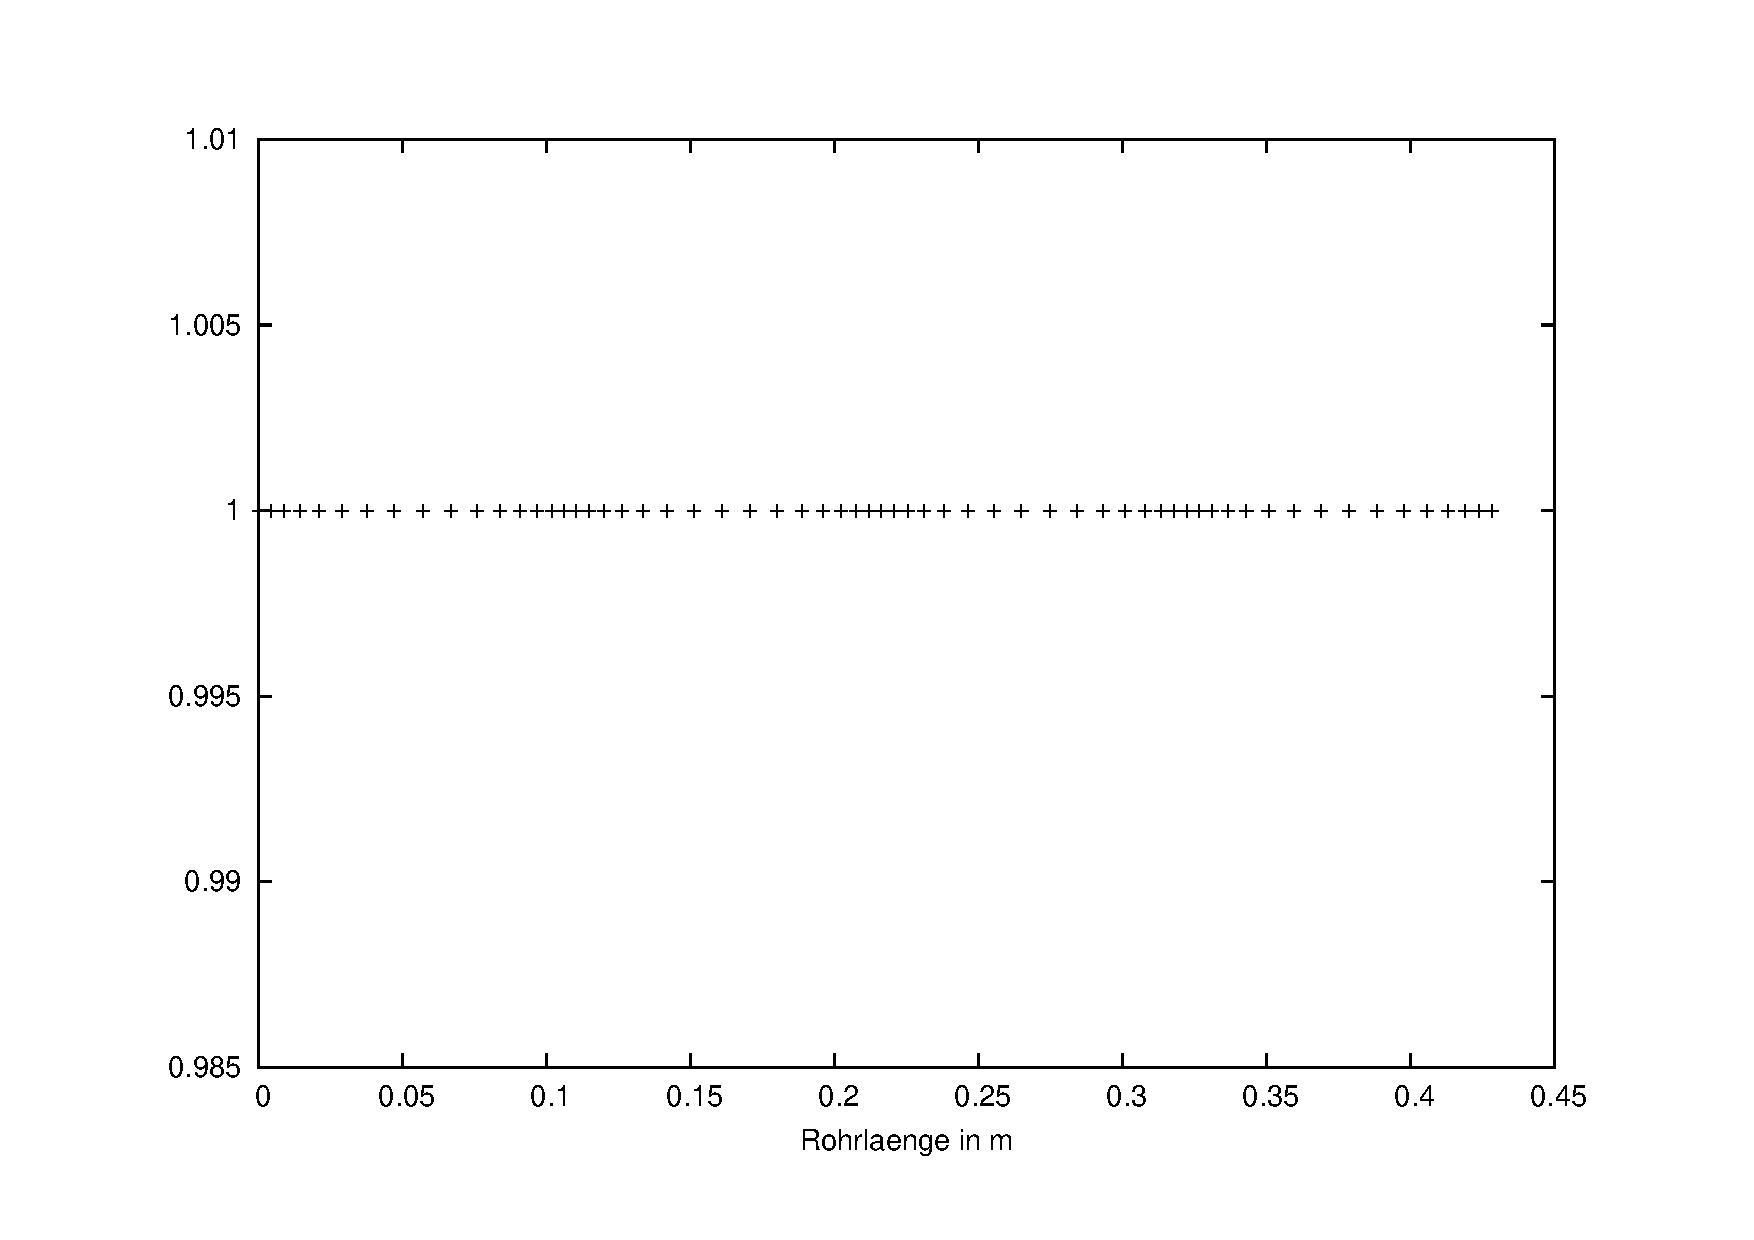
\includegraphics[width=0.9\textwidth]{praktika/mat_praktika/long01}\label{s_t0}}


\subfigure[Hier sind sie in Ruhelage gezeigt (bspw. \(t = \frac{T}{4}\))]{
	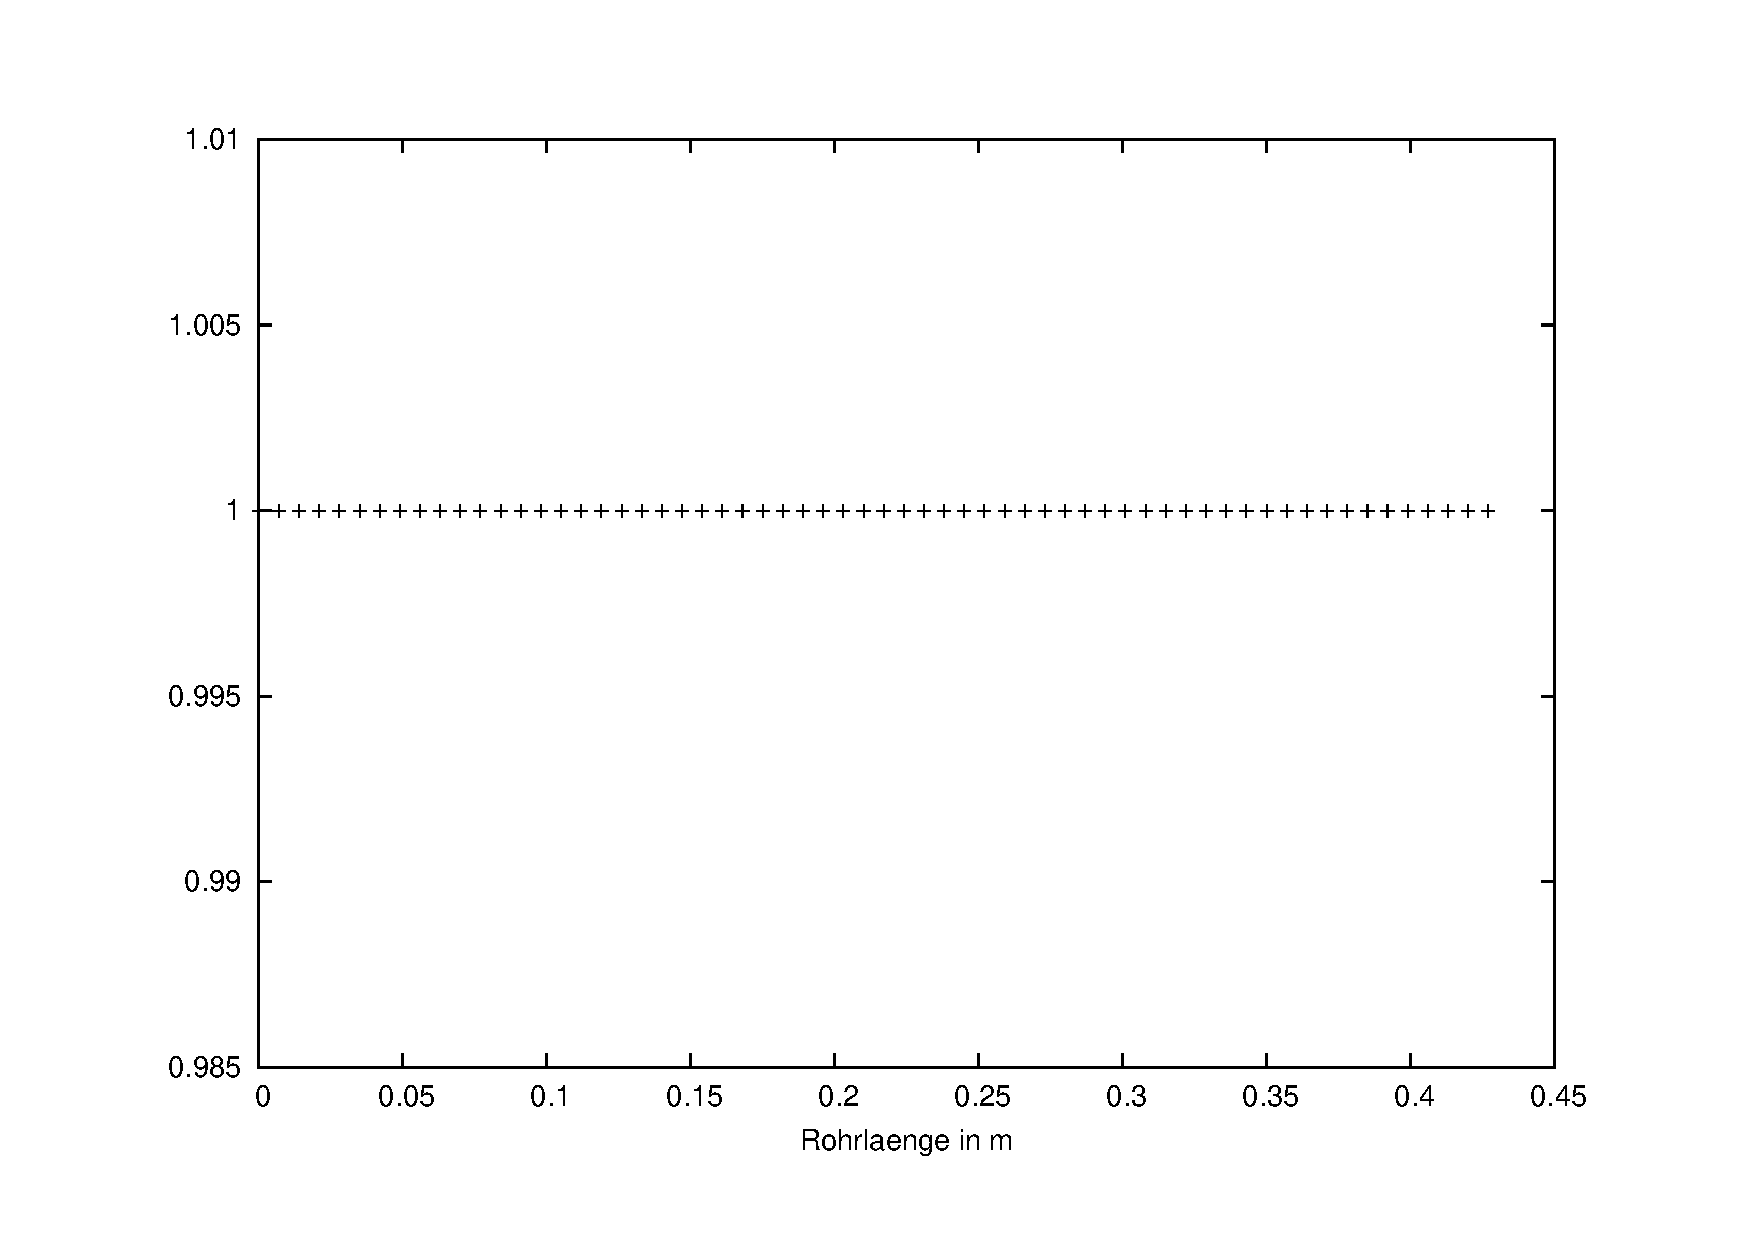
\includegraphics[width=0.9\textwidth]{praktika/mat_praktika/long02}\label{s_t1}}

\caption{In diesem Schaubild sind Luftteilchen eingezeichnet, die in der Ruhelage alle 7mm voneinander entfernt liegen würden. Bei \(x = 0\) kann man sich den Stopfen vorstellen.}
\label{s}
\end{figure}


\begin{figure}
	\centering
 	\subfigure[Die Teilchen bei maximaler Auslenkung (bspw. \(t = 0\))]{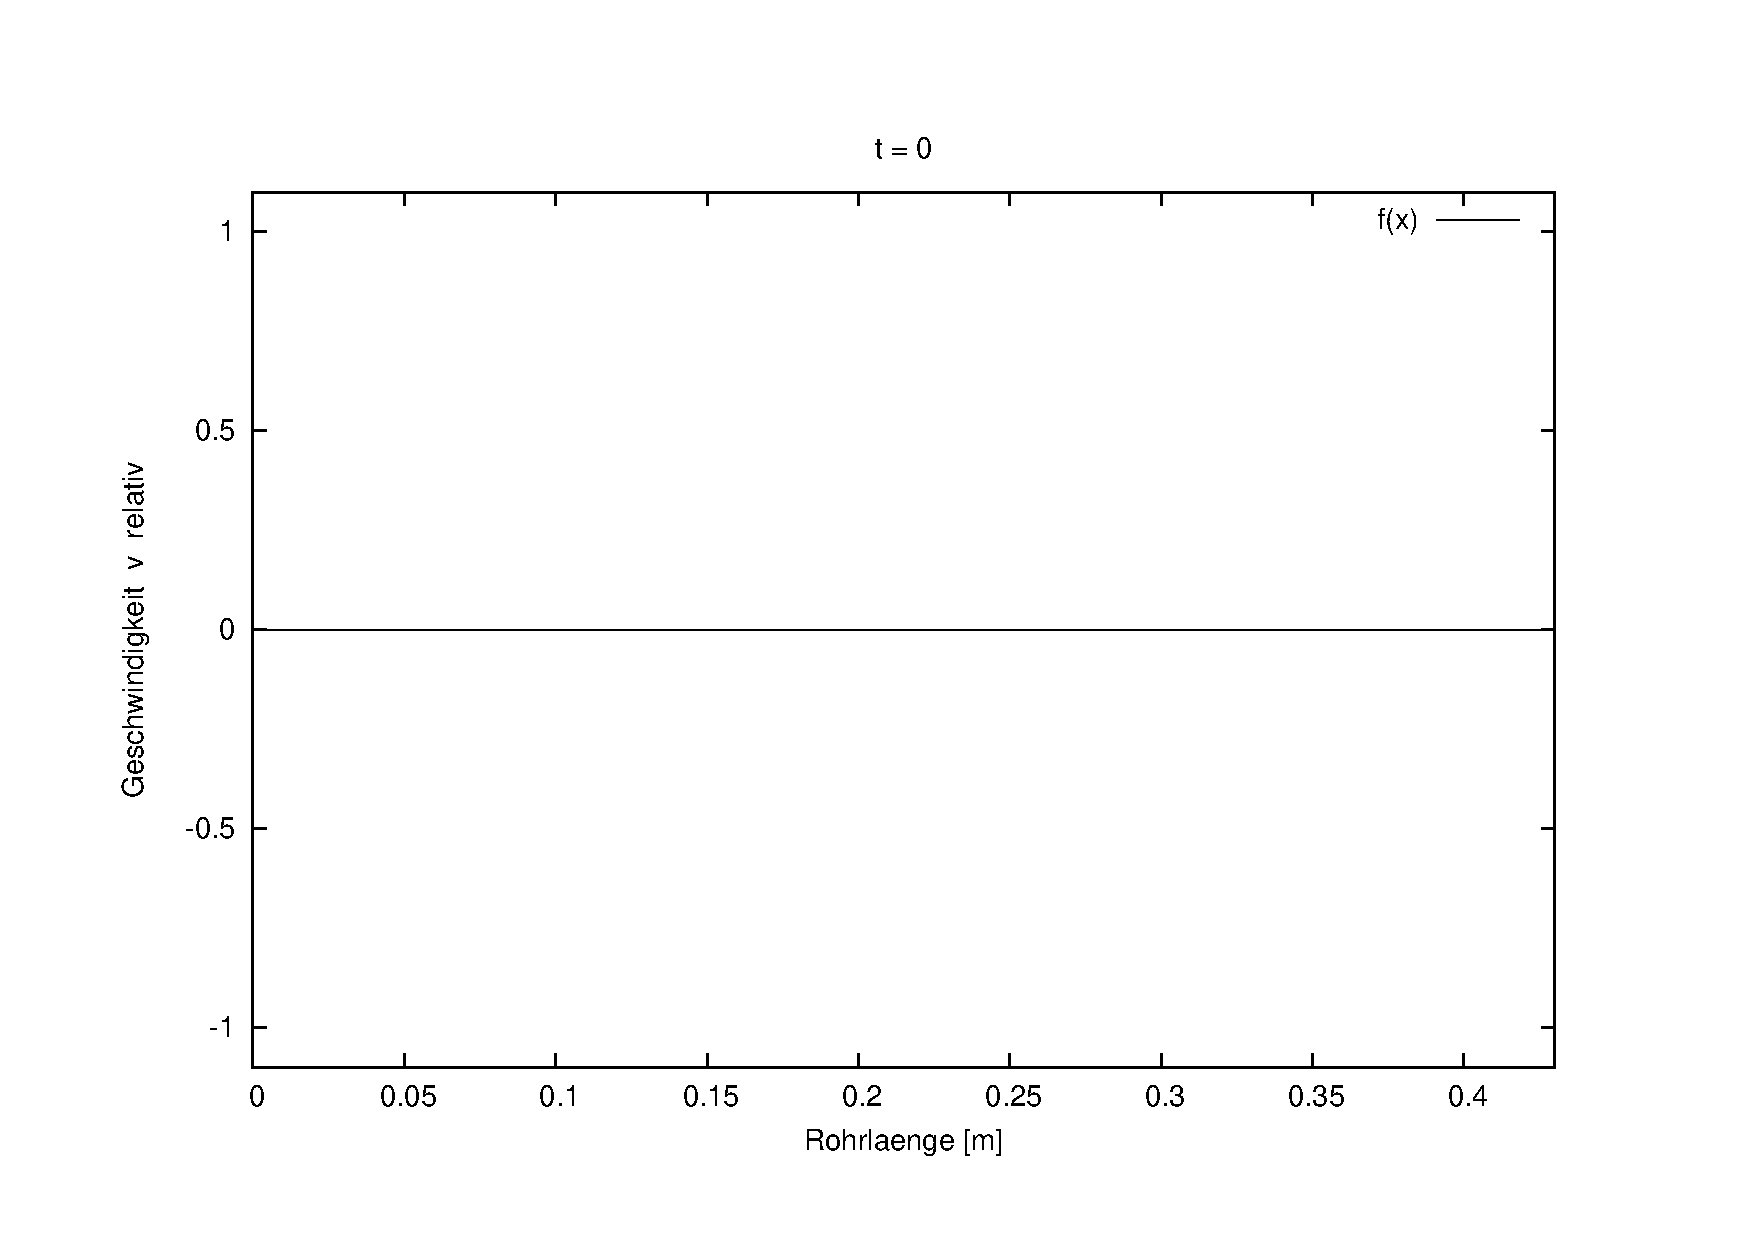
\includegraphics[width=0.9\textwidth]{praktika/mat_praktika/ges01}\label{v_t0}}

	\subfigure[Die Teilchen in Ruhelage (bspw. \(t = \frac{T}{4}\))]{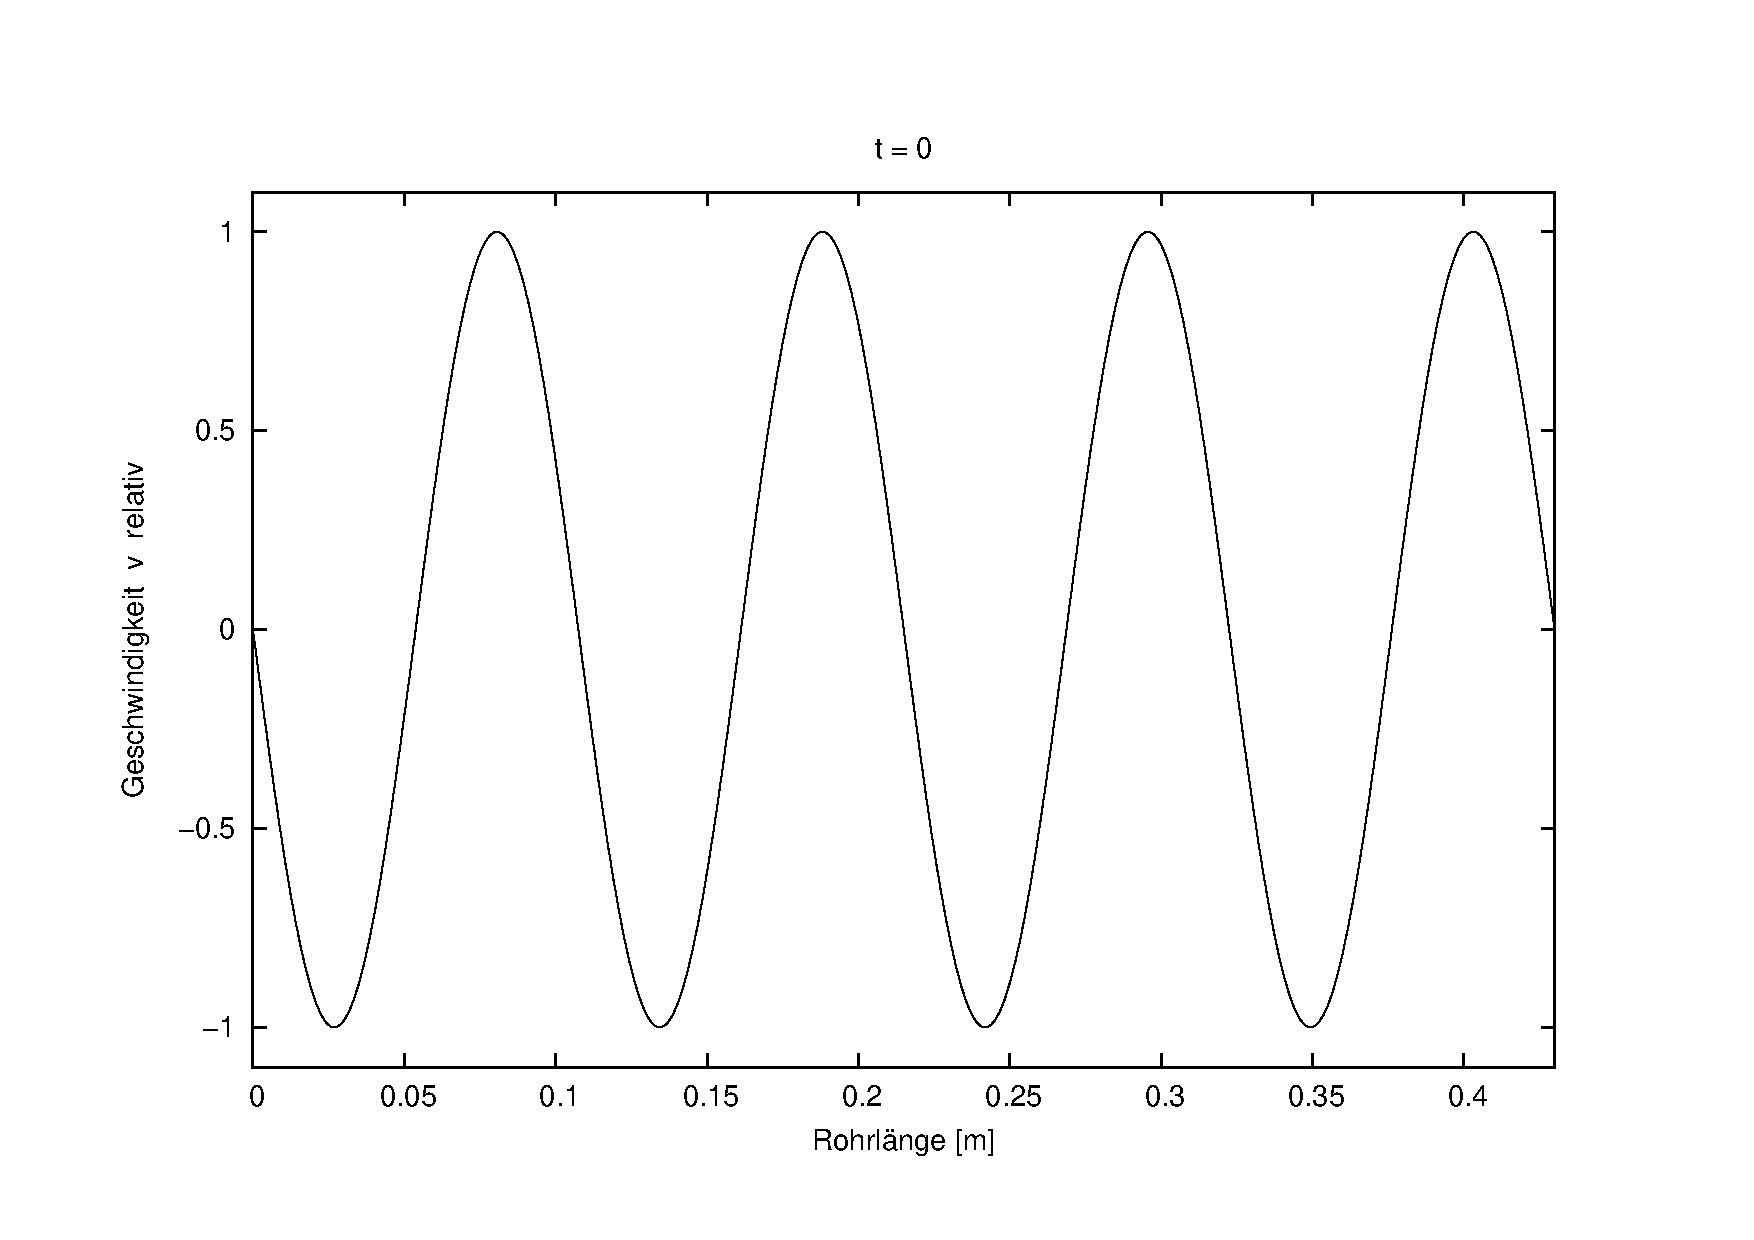
\includegraphics[width=0.9\textwidth]{praktika/mat_praktika/geschw02}\label{v_t1}}

	\caption{Hier sind die relativen Geschwindigkeiten der Luftteilchen eingetragen.}\label{v}
\end{figure}


\begin{figure}
	\centering
 	\subfigure[Die Teilchen bei maximaler Auslenkung (bspw. \(t = 0\))]{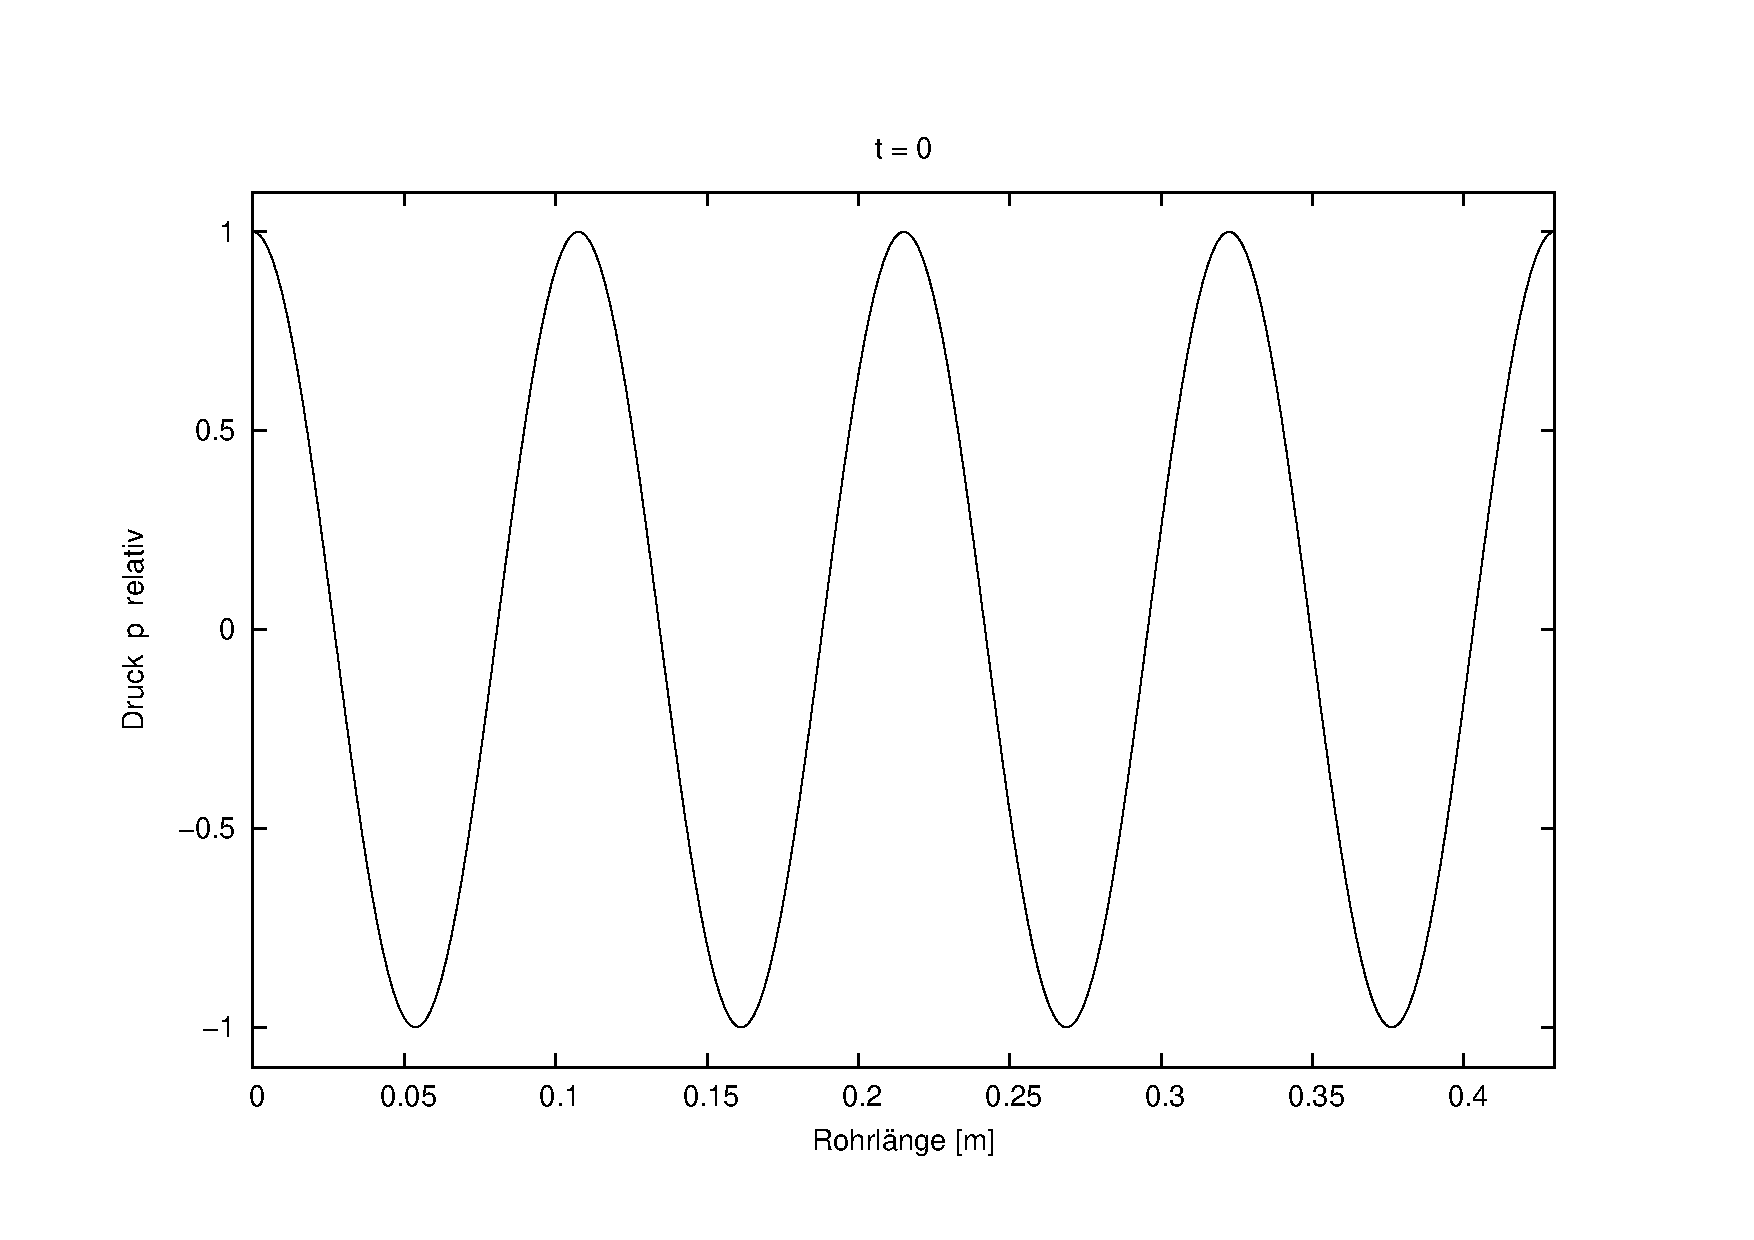
\includegraphics[width=0.9\textwidth]{praktika/mat_praktika/druck01}\label{p_t0}}

	\subfigure[Die Teilchen in Ruhelage (bspw. \(t = \frac{T}{4}\))]{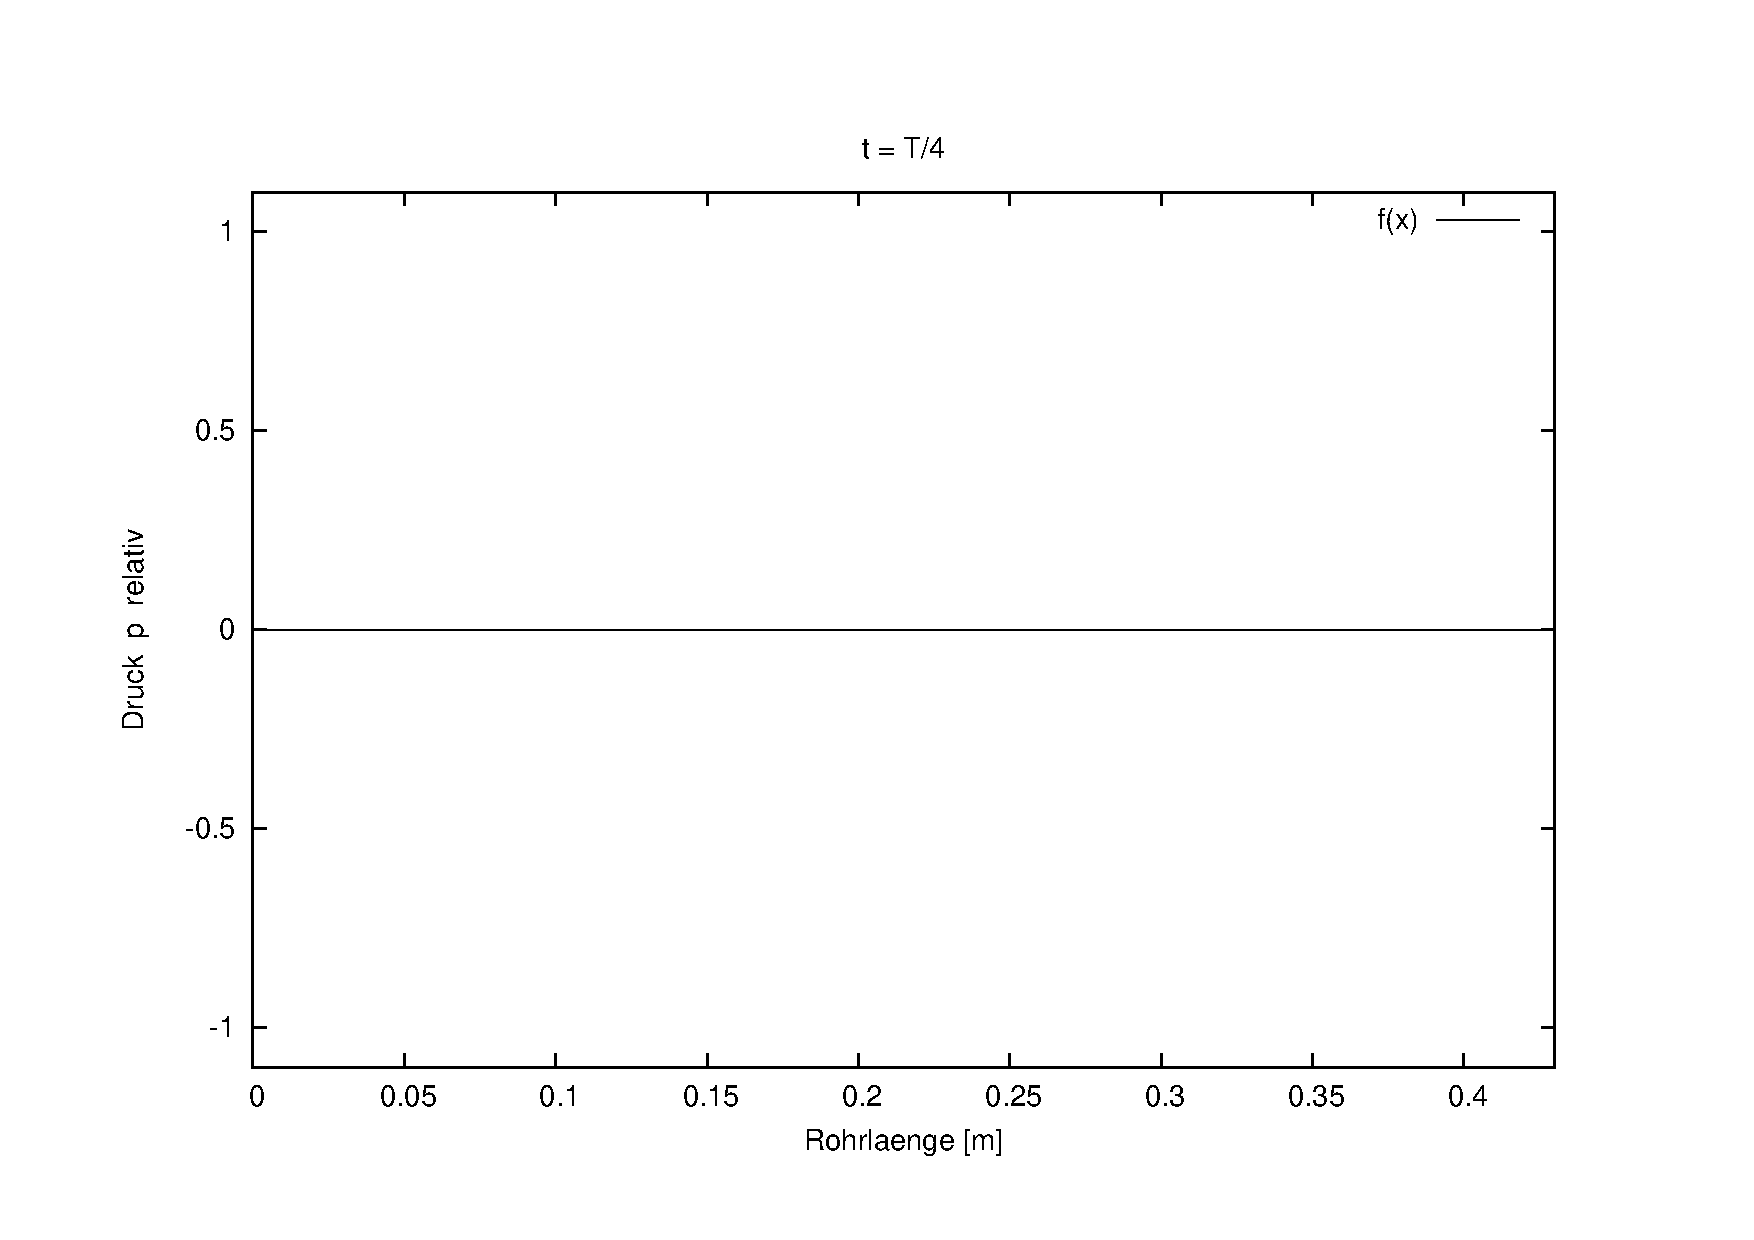
\includegraphics[width=0.9\textwidth]{praktika/mat_praktika/dru02}\label{p_t1}}

	\caption{Hier sind die relativen Drücke der Luft eingetragen.}\label{p}
\end{figure}


\clearpage



		\section{Schallgeschwindigkeit in Messing}

Nun wird auf das noch offene Ende des Resonanzrohres das Erregerrohr aus Messing aufgesetzt. Genau in der Mitte wird es eingespannt. An dieser Stelle ist also gewissermaßen ein Geschwindigkeitsknoten erzwungen. Die Enden des Stabes dagegen können (ziemlich\footnote{An der Stelle mit dem Kopplungskork zwar weniger, es handelt sich hier aber nicht um ein feste Ende, weil der Kork so ausgelegt ist, die Bewegung des Messingrohres weiterzuleiten - er darf sie also nicht bremsen.}) frei schwingen. 

Durch die Anregung des Rohres mit einem nassen Lappen dürften sich Transversalstörungen und sogar Transversalwellen bilden. Diese dürften dann an den Enden des Messingrohrs reflektiert werden\footnote{teilweise werden sie am Kopplungskork an die Luftsäule abgegeben}. Somit müsste sich im Messingrohr eine stehende Transversalwelle bilden. Durch die vorgegebenen Bedingungen\footnote{an den beiden freien Enden Schwingungsbäuche und in der Mitte ein Schwingungsknoten} kann das Rohr nur in bestimmten Frequenzen mit einer stehenden Welle schwingen - nämlich nur dann, wenn sich nach der entsprechenden Wellenlänge und der Formel
	\begin{equation}
 	L = k \cdot \frac{\lambda_k}{2}
	\label{2offen}
\end{equation}
\emph{ungerade} \(k\) ergeben\footnote{also \(k = (1;3;5;...)\)}. Das Rohr kann also in seiner Grundschwingung (1. Harmonische) schwingen, dann aber erst wieder in der 3. Harmonischen, aber nicht in der 2. Harmonischen (der \emph{Oberschwingung}).


Ist die Länge \(L_{mess}\) des Messingrohres bekannt, so kann man damit die Schallgeschwindigkeit in Messing berechnen. Hierzu versetzt man das Messingrohr in Schwingungen, bis sich eine harmonische Schwingung ergeben hat. Bei dieser zählt man dann die \textit{Wellenknoten} - diese Anzahl ergibt den Faktor \(k\). Die Frequenz \(f\), mit der das Messingrohr schwingt, muss man so herausfinden wie in Kapitel \ref{kap:c_luft}.

Schwingt das Messingrohr also, stellt man den Abstimmstopfen so ein, dass sich die Korkspähne im Rohr wieder zu Hügelchen anordnen. Zwischen diesen misst man dann die Abstände und damit \(\frac{\lambda}{2}\). Über die schon vorher errechnete Schallgeschwindigkeit in Luft \(c\) kann man so nach Formel \ref{c_luft} einfach die Frequenz bestimmen, mit der die Luftsäule schwingt. Sie ist genauso groß, wie die Frequenz, mit der das Messingrohr schwingt - in unserem Falle war \(\lambda = 0,1434m\), somit ergibt sich
	\begin{equation}
 f_{mess} = \frac{c}{\lambda} = \frac{365,5\frac{m}{s}}{0,1434m} = 2548,8 \frac{1}{s} \approx 2,55 kHz
\end{equation}
Über die Zusammenhänge aus Formel \ref{c_luft} und \ref{2offen} ergibt sich für die Schallgeschwindigkeit in Messing bei einem Messingrohr der Länge \(L_{mess} = 0.67m\), das mit einem einzigen Wellenknoten (\(k = 1\)) mit der Frequenz \(f_{mess} = 2548,8 Hz\) schwingt die Schallgeschwindigkeit
	\begin{equation}
 	c_{mess} = \frac{2 \cdot f_{mess} \cdot L_{mess}}{k} = 2 \cdot 2548,8 \frac{1}{s} \cdot 0,67m = 3415,4 \frac{m}{s}
	\label{causf}
\end{equation}
Diese Berechnung war sehr präzise - der Literaturwert liegt bei \(3400 \frac{m}{s}\), das ergibt eine Abweichung von \(0,45\%\).


~\\


Ironischerweise befindet sich der Kopplungskork dabei an einem Geschwindigkeits\emph{knoten}. Das ist aber leicht zu erklären, weil es sich bei dem Kork ja immer noch um ein festes Ende handelt, das bei einer stehenden Welle eben \emph{immer} einen Geschwindigkeitsknoten hervorruft. 

Gleichzeitig ist an der Stelle aber ein \emph{Druckbauch}. Das ist nun wieder leicht zu verstehen und auch bildhaft vorzustellen: Der Kopplungskork wandelt die Transversalwellen des Messingrohres in Longitudialwellen um. Dabei drückt er die direkt vor ihm liegende Luft abwechselnd zusammen (erzeugt also Überdruck), um dann wieder beim Zurückweichen einen Unterdruck zu erzeugen (der die Teilchen wieder auseinander zieht). Die Teilchen direkt am Kork werden dabei aber wenig bewegt; sie geben praktisch nur den Druck weiter.




		\section{Erregung mit Lautsprecher}


Nun werden beide Enden des Rohres frei gemacht und ein Lautsprecher wird vor eines der beiden offenen Enden positioniert. Er hat etwas Abstand zum Rohr, damit sich hier kein geschlossenenes Ende ergibt. Nun wird der Lautsprecher an einen Sinusgenerator angeschlossen und bei diesem wird die Frequenz so lange geändert, bis sich die bereits beobachteten Resonanzphenomäne einstellen - bis der Kork sich also wieder in Häufchen anordnet. Ist das geschehen, wird die Frequenz möglichst präzise gemessen - dazu verwendet man ein Mikrophon, das an ein Oszilloskop angeschlossen wird. Das Mikrophon kann man hinter dem zweiten offenen Ende des Rohes positionieren; auch wenn der Schall hier eigentlich in das Rohr zurück reflektiert wird, werden stets genügend Luftteilchen in der Umgebung mit angeregt, um den Schall aus dem Rohr hinauszutragen.

Diese Messung ergab eine Frequenz von \(f_{anr} = \frac{1}{0,0012s} \approx 833,3Hz\). Da de stehende Welle hier aufgrund der Bedingung zweier loser Enden zustande gekommen ist, kann man Formel \ref{2offen} heranziehen, wobei diesmal alle positiven, ganzzahligen \(k\) erreicht werden dürfen.\footnote{\(k = (1; 2; 3; ...)\)} Durch abzählen der \textit{Geschwindigkeitsbäuche} (also der Stellen, an denen \emph{kein} Kork liegt) erhält man den Faktor \(k\) - in unserem Falle ist \(k = 2\). Die Länge des Rohres beträgt \(L_{Rohr} = 0,43m\). Wir können hier die Umformung von Formel \ref{causf} verwenden\footnote{Die Formel aus den Bedingungen ``zwei offene Enden'' ist die selbe wie für die Bedingungen ``zwei geschlossene Enden''.}. Es ergibt sich für uns also:
\begin{equation}
 	c_{Luft} = \frac{2 \cdot f \cdot L_{Rohr}}{k} = \frac{2 \cdot 833,3\frac{1}{s} \cdot 0,43m}{2} = 358,319\frac{m}{s}  \approx 358 \frac{m}{s}
\end{equation}
und damit eine Abweichung von \(4,4\%\) zum Literaturwert und eine Abweichung von \(-2,2\%\) zu dem Wert, den wir vorher errechnet hatten.

% literatur: 	343
% 1. Versuch:	366



		\section{Zusammenfassung}

Für die Schallgeschwindigkeiten haben wir also mit verschiedenen Möglichkeiten folgende Werte errechnet:

\begin{table}[h]

\centering
 	\begin{tabular}{| c | c | c | c |}
\hline
Medium & Methode (Reflexionsbedingungen) & Wert & Abweichung v. Literatur \\
\hline
\hline

Luft & Stimmgabel, (offen, geschlossen) & \(366\frac{m}{s}\) & \(6,6\%\) \\

Luft & Lautsprecher (offen, offen) & \(358\frac{m}{s}\) & \(4,4\%\) \\

Messing & Erregerrohr (offen, offen) & \(3415\frac{m}{s}\) & \(0,5\%\) \\

\hline

\end{tabular}

\caption{Zusammenstellung der Messergebnisse}

\end{table}


Diese Ergebnisse zeigen, dass wir sehr präzise gearbeitet haben. Die geringen Abweichungen lassen sich sicher dadurch erklären, dass wir bspw. die Länge der Röhre nicht präzise genug messen konnten - schließlich wird nicht die gesamte Röhre als Resonanzkörper verwendet; der Stopfen ragt ja etwas hinein.

Ein weiteres Problem könnte sein, dass der Stopfen nicht hart genug war. Sowohl der Kopplungskork als auch der Abstimmstopfen sind aus Materialien, die sich minimal von der Luftsäule mitbewegen lassen. Die Enden sind also nicht \(100\%\)ig fest.

Auch die Beschriftung der Stimmgabel muss nicht völlig korrekt gewesen sein; schon kleine Abweichungen der tatsächlichen Frequenz von der, die wir zur Berechnung verwendet haben, haben schon große Auswirkungen.

Darüber hinaus muss der Literaturwert der Schallgeschwindigkeit nicht mit dem \emph{tatsächlichen} Wert überein\-stimmen - eigentlich hätte man Bedingungen wie Temperatur, Luftfeuchtigkeit etc. einrechnen müssen, darüber hinaus können die Medien ``\textit{verschmutzt}'' sein, dass also Teile anderer Stoffe enthalten sind, die die Schallgeschwindigkeit beeinflussen können.

Eine weitere Ungenauigkeit könnte sich dadurch ergeben, dass die von uns beobachtete Welle nicht unbedingt völlig \textit{stehend} war. Möglicherweise können die Resonanzphenomäne teilweise schon beobachtet werden, wenn die Resonanz nicht perfekt ist, und wir haben schon bei solchen nicht perfekten Zuständen die Messwerte genommen.



%\end{document}
